\documentclass{article}
\usepackage{amsmath}
\usepackage{graphicx}

\title{PART-1(Bias-Variance Tradeoff in Machine Learning)}
\author{}
\date{}

\begin{document}

\maketitle

\section*{Impact of Increasing Model Complexity on Bias and Variance}

As we increase the complexity of a machine-learning model by adding more features or including higher-order polynomial terms in a regression model, the effects on bias and variance can be described through the **bias-variance tradeoff**.

\subsection*{1. Bias}
Bias refers to the error introduced by approximating a real-world problem with a simpler model. 

- Low-complexity models (e.g., linear models) typically have \textbf{high bias}, as they underfit the data and fail to capture underlying patterns.
- As model complexity increases, bias \textbf{decreases}, since the model can fit more complex patterns.

\subsection*{2. Variance}
Variance refers to the model's sensitivity to small fluctuations in the training data.

- High-complexity models, especially those with many features or higher-order terms, have \textbf{high variance} since they can overfit the training data, learning patterns that do not generalize well to unseen data.
- As model complexity increases, variance \textbf{increases}, as the model becomes too sensitive to the specific training data.

\subsection*{3. Bias-Variance Tradeoff}
The bias-variance tradeoff represents the balance between bias and variance:

\begin{itemize}
    \item Initially, as complexity increases, both training and test errors decrease due to a reduction in bias.
    \item After a certain point, increasing complexity results in overfitting, which causes an increase in test error due to higher variance.
\end{itemize}

\section*{Graphical Representation}

The bias-variance tradeoff can be represented graphically as shown below:

\begin{center}
    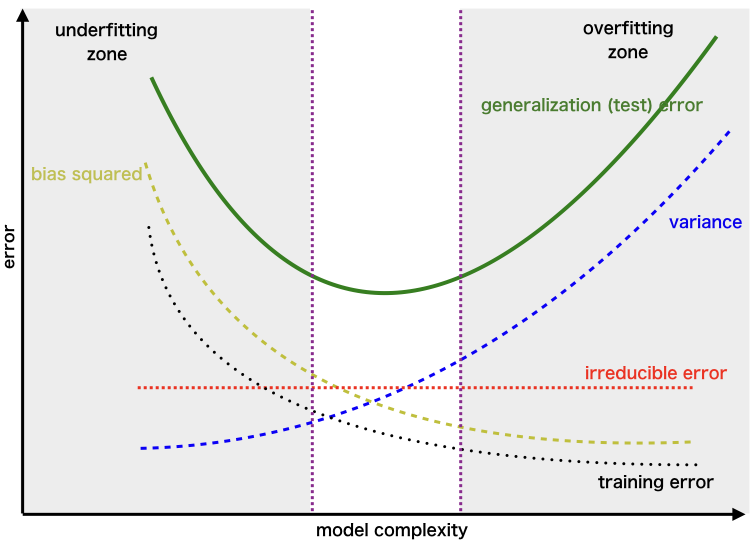
\includegraphics[width=0.6\textwidth]{bias-variance.png}
\end{center}

In this graph:
- The \textbf{x-axis} represents model complexity.
- The \textbf{y-axis} represents the error (or loss).
- The \textbf{training error} decreases as complexity increases.
- The \textbf{test error} initially decreases but then increases due to overfitting.
- \textbf{Bias} starts high and decreases, while \textbf{variance} starts low and increases.

\subsection*{Mathematical Formulation}

The total error can be decomposed into three parts:

\[
\text{Total Error} = \underbrace{\text{Bias}^2}_{\text{underfitting}} + \underbrace{\text{Variance}}_{\text{overfitting}} + \underbrace{\text{Irreducible Error}^2}_{\text{Noise}}
\]

- \textbf{Bias}: Measures how far the model's predictions are from the true values.
- \textbf{Variance}: Measures the model's sensitivity to changes in the training data.
- \textbf{Irreducible error}: Represents the inherent noise in the data.

% \section*{Conclusion}

% In summary, as model complexity increases, bias decreases and variance increases. There exists an optimal point of complexity that minimizes the test error, balancing bias and variance.

\end{document}
